\section{Implementation}
\label{sec:impl}

\subsection{WebOS vs Android}
\Comment{ADD MORE HERE}
\subsubsection{libc vs bionic}
Despite the fact the Pre and the Android are both running Linux OSes on an ARM chip, the environments they provide for our project are enormously different.  The Pre is bundled with a large suite of common Unix applications and libraries, while the Android diverges, running minimalistic libraries and lacking many common libraries and applications.  Of these differences, the C compiler library is probably the most substantial. The Pre uses an unmodified version of glibc and the Android uses Bionic, a lightweight and small C compiler library.  Many Linux applications have glibc as a dependency, and as a result, builds for the Android must have statically link libraries.  Between this and the lack of useful applications (gdb and other debugging tools) development on the Android has proven much more difficult.  \\

\subsection{LXC and module compatibility}

\Comment{CLEANUP}
While experimenting with new kernels on our WebOS devices, we encountered an issue that took some work to get around.  Like many mobile devices the Palm Pre ships with a number of binary modules for which the source is unavailable.  For example, the wifi drivers ``sd8xxx.ko'' and ``uap8xxx.ko'' ship with the device, but are not open-source and so all we have is the final binary module.  This is not uncommon for linux drivers, but presents us with two issues, both having to do with maintaining the ABI. \\

    The first issue is simpler, regarding the 'MODVERSIONS' config option in the kernel \Comment{CITE}.  This config option serves the purpose of help identify symbols by their contents and functionality by appending a CRC of related information to the symbol name.  This was an issue because our changes modified slightly (if not functionally) the definitions of some code, and resulted in mismatched version info.  Our solution was to build the kernel without support for this, but the result is less safe checking of loaded modules.  Note that this is not a security concern since loading modules is a privileged operation anyway, but rather is undesirable to help prevent the careless user from loading modules they should not. \\

    The second issue is similar but presented more of a challenge was what this locking to a particular ABI meant regarding the kinds of changes we could make.  The Pre ships with a modified version of linux 2.6.24 \Comment{CITE}, but full support for LXC was not merged into the linux mainline until 2.6.26 \Comment{CITE}.  In 2.6.24 there is partial LXC support, and we had to backport some of the other pieces.  However we were unable to get full LXC support since some features (such as network namespaces) are rely on significant changes in the kernel architecture.  However, this is not a fault in our design and a device manufacturer most likely would not be faced with this issue, being in the position to acquire or build the related modules for the kernel version they desired. \\


\subsection{X-Server}

The X-server serves as the graphical framework that integrates the applications into the host environment.  As part of our efforts to bring X11 to the phones, we had to make a few decisions that are detailed below. \\

\subsubsection{DDX}
The X-Server architecture contains multiple Device Dependent X (DDX) implementations.  The most used one is `xfree86', but there are others, such as `kdrive' \cite{x_glossary}.  We chose to use kdrive because of the Xsdl functionality it contains, which allows one to run X using SDL as a backend.  Unfortunately Xsdl is so out of date that it was recently removed from the X project altogether due to being broken and unmaintained. \\

From X version control: ``if anyone uses this in production, a big scary monster will eat them'' \cite{x_quote}.  The unfortunate result of this was much work spent fixing Xsdl and bringing it up to date, in order to work with the rest of X.  Fixes including interactions with the X server, as well as fixing the rendering code and the input handling. \\

\subsubsection{SDL and GLES}
As described above, the code we started with \Comment{Palm Pre code or kdrive code?} used Simple DirectMedia Layer (SDL) \cite{sdl} for input and rendering.  Once we had achieved this functionality, we noticed the display lagged when doing even basic things like moving the cursor.  Previous experience working with SDL on this device suggested that using GLESv2 \cite{gles} and custom shaders would improve a task even as simple as blitting \Comment{define}, so we ported the rendering bits to use GLESv2. \\

\subsubsection{Devices that do not support SDL}
Although the Pre has support for SDL, many devices do not, and that is something we have taken into consideration.  The kdrive structure can be made rather portable: at its heart it just needs something that can render a pixelbufer, and feed it input (either event driven or by polling).  This means that we could potentially support Android devices through Java Native Interface (JNI) \cite{jni} passing the buffer to a java application to blit and the java application blitting to the screen, as well as gathering input and feeding it to the X server. \\

\subsubsection{Keyboard}
Keyboard support is very important when using applications.  However it was a stumbling block for us for two main reasons: 1) mapping SDL to something the X server can use 2) adding support for keys and features that are not on the original device.\\

It is common for keyboards, particularly on phones, to have each key have multiple uses when pressed with a special modifier.  As an example, on the Pre, `orange' plus `q' is the `/' key.  This presented a problem because this means capturing the modifier requires creating a state machine to process the input as opposed to a simple lookup table.  We ended up using xkb to do this, and the results are in the xkeyboard-config git repository. \\

The second issue is that many keys that are required for doing something as simple as using `xterm' simply do not exist on most phones.  Examples of such characters include the pipe `\textbar' character, `\textgreater', `\textless', arrow keys, and more.  We currently support many such keys on the Pre through more customizations to the xkb layout and hope to support other devices as we add support for them as well. \\

\subsubsection{Future: Integrating even more}
A primary goal of our project is to cleanly integrate into the host X server.  While our current implementation is a great step and does integrate as a window in the existing windowing system for the device, there is an issue.  Presently the X server will render everything into one window (see Figure \ref{fig:x_screenie}), which requires a window manager to manage the windows.  This is bad both because it is hard to use but also because it is a hard break from the goal of integrating with the parent window manager--now the user has to think about it as two separate systems.\\

One solution to this is to take advantage of the work done on rootless X \cite{rootless}.  ``The generic rootless layer allows an X server to be implemented on top of another window server in a cooperative manner. This allows the X11 windows and native windows of the underlying window server to coexist on the same screen. The layer is called ``rootless'' because the root window of the X server is generally not drawn. Instead, each top-level child of the root window is represented as a separate on-screen window by the underlying window server'' \cite{rootless}.\\

Another idea is to take advantage of standard X notification events \cite{notifications} and hook into mobile device notification systems, which both WebOS and Android support. \\

\begin{figure}[tbh]
\centering
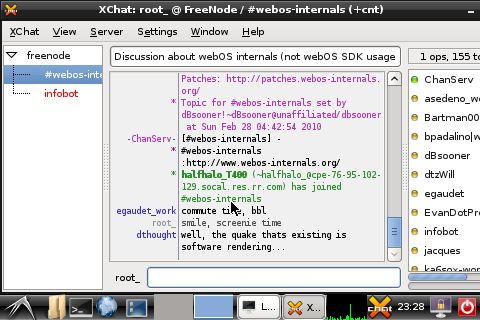
\includegraphics[width=1.0\columnwidth]{xchat1}
\caption{X server running icem and xchat}
\label{fig:x_screenie}
\end{figure}
